%=================================================================
% Two Streams, Four Architectures — MDPI MTI submission
% Built on the official MDPI template (Definitions/mdpi.cls, unmodified).
% Nothing under Definitions/ may be edited.
%=================================================================
\documentclass[mti,article,submit,moreauthors]{Definitions/mdpi}

%=================================================================
% MDPI internal commands - do not modify
\firstpage{1}
\makeatletter
\setcounter{page}{\@firstpage}
\makeatother
\pubvolume{1}
\issuenum{1}
\articlenumber{0}
\pubyear{2026}
\copyrightyear{2026}
\datereceived{ }
\daterevised{ }
\dateaccepted{ }
\datepublished{ }
\externalbibliography{yes}

% Float placement. LaTeX's defaults reserve so much of each page for text that a
% page carrying two large floats is left half empty; across six figures and five
% tables that costs several pages of white space. These are the standard
% relaxations: they change only where floats are allowed to sit, never the
% typography, the content, or the class file.
\renewcommand{\topfraction}{0.92}
\renewcommand{\bottomfraction}{0.85}
\renewcommand{\textfraction}{0.06}
\renewcommand{\floatpagefraction}{0.80}
\setcounter{topnumber}{3}
\setcounter{bottomnumber}{2}
\setcounter{totalnumber}{4}

%=================================================================
% Full title of the paper (Capitalized)
\Title{Two Streams, Four Architectures: A Leakage-Free, Statistically Rigorous Benchmark for Pedestrian Crossing-Intention Prediction on PIE}

% Author Orchid ID: enter ID or remove command
\newcommand{\orcidauthorA}{0000-0000-0000-0000} % PLACEHOLDER

% Authors, for the paper (add full first names)
\Author{PLACEHOLDER Firstname Lastname $^{1,}$*\orcidA{} and PLACEHOLDER Firstname Lastname $^{1}$}

% MDPI internal command: Authors, for metadata in PDF
\AuthorNames{PLACEHOLDER Firstname Lastname, PLACEHOLDER Firstname Lastname}

% Affiliations / Addresses
\address{%
$^{1}$ \quad PLACEHOLDER Department, PLACEHOLDER University, PLACEHOLDER City, PLACEHOLDER Country; placeholder@example.com}

% Contact information of the corresponding author
\corres{Correspondence: placeholder@example.com}

% Abstract — written last (S9)
\abstract{Predicting whether a pedestrian is about to cross is a core requirement for automated vehicles, and the PIE dataset is its standard testbed. We first show that the observation windows commonly extracted from PIE contain the event they are meant to precede: measured against the dataset's own per-frame crossing annotation, 67.9\% of crossing sequences are observed while the pedestrian is already crossing. Re-anchoring every window at the labelled crossing event, with a minimum look-ahead of thirty frames, removes this by construction and yields 3.5 times as many windows. On the re-extracted data we evaluate a deliberately minimal model that sees only a pedestrian bounding box and the ego-vehicle speed over sixteen frames, and we compare four temporal encoders, an LSTM, a Transformer, a GRU and an un-gated Elman RNN, trained through one engine at matched and at separately tuned configurations under equal search budgets. The four reach F1 between 0.844 and 0.852 and ROC-AUC between 0.940 and 0.948, and are statistically indistinguishable on F1 under a pedestrian-cluster bootstrap. Removing ego speed drops F1 to 0.551. The input signal, not the temporal architecture, determines performance on this task.}

% Keywords — written last (S9)
\keyword{pedestrian crossing intention; pedestrian behaviour prediction; data leakage; benchmark protocol; PIE dataset; recurrent neural networks; transformers; advanced driver assistance systems; model comparison; bootstrap confidence intervals}

%=================================================================
\begin{document}

\section{Introduction}
\label{sec:introduction}

For an automated vehicle, a pedestrian who has been detected is only half of the problem. It also has to anticipate whether that person is about to enter its path, early enough for the answer to be worth acting on. Consider someone stepping off the kerb from between parked cars on an urban street after dark. A vehicle travelling at 50~km/h covers about 14~m every second, so the road left for braking is set by the moment the vehicle judged that this person was about to cross, and half a second of hesitation costs about 7~m of it. The pedestrian gives no advance notice of the decision to cross. There is no traffic signal to read, no marked crossing to step onto, and usually no glance towards the driver. That leaves motion as the only evidence available: how the pedestrian is moving, and how fast the vehicle is closing, in the seconds before that first step. Figure~\ref{fig:scenario} shows the last two seconds of one such approach, recorded in PIE.

\begin{figure}[H]
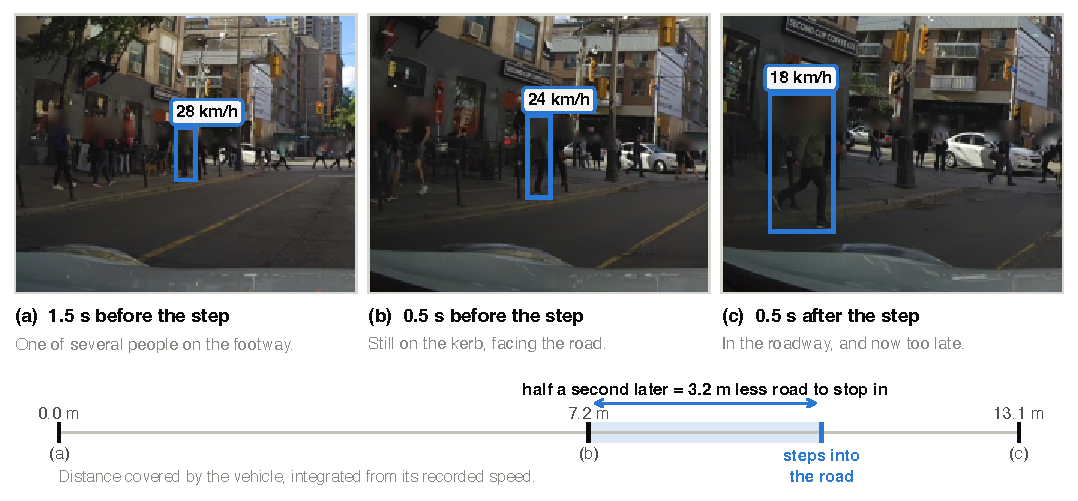
\includegraphics[width=\textwidth]{figures/fig_scenario.pdf}
\caption{What the vehicle sees before a crossing, and what a delay costs, on a real PIE sequence (video 0016, pedestrian 3\_16\_919). Panels give the ego-vehicle view 1.5\,s and 0.5\,s before this pedestrian stepped into the road, and 0.5\,s after; boxes are the dataset's own annotations and the speeds its recorded ego-vehicle channel. In (\textbf{a}) the subject is one of several people on that footway and nothing in the image separates them from those who stay put, while by (\textbf{c}) the decision is unambiguous and the vehicle has travelled 13.1\,m. The half second between (\textbf{b}) and the step accounts for 3.2\,m of that; at the 50\,km/h of a typical urban limit the same half second would cost about 7\,m. Distances are integrated from the recorded speed. Head regions were irreversibly blurred before publication.\label{fig:scenario}}
\end{figure}

That scene is an ordinary one. Figure~\ref{fig:stats} gives the scale. Road traffic crashes killed about 1.16 million people in 2025, and they remain the leading cause of death for people aged 5 to 29~\citep{who2026factsheet,who2026roaddeaths}. The global death rate has fallen by 21\% since 2011, yet pedestrians remain 23\% of the toll, the second largest group after occupants of four-wheeled vehicles~\citep{who2023roadsafety}. United States data show it more closely. Pedestrian deaths there peaked at 7,593 in 2022 and have fallen since, reaching 7,080 in 2024~\citep{nhtsa2026pedestrians}. The direction is right, but the level is not: the 2024 figure is still 29\% above the 5,494 of 2015, and across that decade pedestrians rose from 15\% to 18\% of all traffic deaths. State-reported data project a further 7\% decline for 2025~\citep{ghsa2026pedestrian}. The circumstances match the scene above rather than a marked crossing: of the 2024 deaths, 84\% were in urban areas, 73\% away from intersections and 76\% in the dark~\citep{nhtsa2026pedestrians}.

\begin{figure}[H]

\includegraphics[width=\textwidth]{figures/fig1_pedestrian_statistics.pdf}
\caption{Pedestrians carry a disproportionate share of road traffic casualties, and one that has come down more slowly than the total. (\textbf{a}) Global road traffic deaths by road user type for 2021, the most recent breakdown by user type published by the World Health Organization~\citep{who2023roadsafety}, whose July 2026 update reports 1.16 million deaths in 2025 but no user-type split. (\textbf{b}) Pedestrians killed in the United States from 2015 to 2024, from the National Highway Traffic Safety Administration's 2024 data~\citep{nhtsa2026pedestrians}. Counts peak in 2022 and fall in the two years after it, while staying well above the level of a decade earlier and rising from 15\% to 18\% of all traffic deaths.\label{fig:stats}}
\end{figure}

Anticipating a crossing in those conditions is the problem this paper works on, and it is narrower than it looks. Crossing-intention prediction asks a binary question about a specific pedestrian at a specific moment: will this person enter the roadway within the next one to two seconds? It is not trajectory forecasting, which asks where an agent will be and is scored by displacement error. The two are related but not interchangeable, and treating them as one has been criticised from inside the field~\citep{rasouli2024diving}. A pedestrian who stands at a kerb for three seconds and then steps out has a nearly stationary trajectory until the moment that matters most. The PIE dataset~\citep{rasouli2019pie} is the standard testbed because it provides what the question needs: over six hours of on-board video, per-frame bounding boxes, synchronised vehicle telemetry, and a labelled crossing event for each pedestrian that fixes when the prediction horizon starts.

Work on that testbed has converged on a shared protocol and a shared design. The benchmark of Kotseruba et al.~\citep{kotseruba2021benchmark} fixed the observation window, the prediction horizon and the split by recording set, and most results published since are reported against it. The models built on it have grown wider, consuming three to seven input streams with pose estimators, optical flow, semantic segmentation or depth behind them~\citep{azarmi2025pipnet,zhou2023pit}, each an extra model to run and a further failure point in a vehicle. Against that trend, one thing this paper does not claim is that minimal inputs are a new idea. Prediction from bounding boxes and ego-vehicle speed alone has been reported before~\citep{chen2024pedcmt,achaji2022attention}, and the pose-free ablation of GTransPDM~\citep{xie2025gtranspdm} demonstrates it within a single paper. Section~\ref{sec:related-work} sets out that precedent in detail.

What that body of work leaves open is method rather than modelling, and three gaps recur across it. The first concerns what the model is shown. Observation windows are commonly anchored at the end of the annotated track, which places no constraint on whether the window overlaps the crossing itself, and no prior study we surveyed measures how often it does; the dataset's own authors note that intention and action samples use different anchors without quantifying the consequence~\citep{rasouli2024diving}. The second is evaluation. Results are typically single point estimates from one split and often one seed, without confidence intervals, cross-set validation, or any account of how much of the reported gap variance alone could produce~\citep{bouthillier2021variance}. The third is the encoder itself, chosen by assertion rather than by test, since no controlled comparison at equal search budgets exists for this task.

Each gap changes what a published number means. A window that contains the crossing scores a model on recognising an event rather than on anticipating it, which is not the capability the application needs. A single point estimate from a single seed cannot separate a real margin between two methods from seed noise. An encoder that is never compared under controlled conditions leaves the field paying for architectural complexity, and for the input streams that feed it, without evidence of what either buys.

This paper closes those three gaps on PIE. We measure the leakage, re-extract the dataset with every window anchored at the labelled crossing event, re-evaluate a deliberately parsimonious two-stream model on the result with interval estimates throughout, and then test whether the choice of temporal encoder matters at all once four families are given the same engine and the same search budget. The contributions are as follows.

\begin{itemize}
\item A quantified audit of temporal leakage in the standard PIE windowing protocol, and a leakage-free re-extraction anchored at the dataset's own crossing event. Under the track-end anchor, 67.9\% of crossing sequences are observed while the crossing is already in progress; the re-anchored protocol contains none, and yields 3.5 times as many windows (Section~\ref{sec:methods}).
\item A re-evaluation of a deliberately parsimonious two-stream model on that protocol, with window-level and pedestrian-cluster bootstrap intervals, leave-one-set-out cross-validation over all six recording sets, multi-seed ablations of horizon, window length and capacity, a documented hyperparameter search, and a detector-in-the-loop test in which the model's inputs come from a detector and tracker in place of annotations (Section~\ref{sec:results}).
\item A controlled comparison of four temporal encoders, an LSTM, a Transformer, a GRU and an un-gated Elman RNN, trained through one engine at a matched configuration and at separately tuned configurations under equal search budgets, which finds them statistically indistinguishable on the primary metric (Sections~\ref{sec:settings} and~\ref{sec:results}).
\end{itemize}

The primary metric named in the third contribution is F1: throughout the paper we report F1 first, then accuracy, then ROC-AUC and PR-AUC. F1 is the operating-point metric appropriate to an imbalanced binary decision where a missed crossing costs more than a false alarm, and the threshold-free measures are reported alongside it as corroboration. Section~\ref{sec:methods} states what that ordering does and does not rest on in the literature.

\section{Related Work}
\label{sec:related-work}

\subsection{Datasets, Benchmarks, and Models}

Two datasets define this task. JAAD~\citep{rasouli2017jaad} supplied the first annotated corpus of pedestrian crossing behaviour from a moving vehicle, and PIE~\citep{rasouli2019pie} added synchronised on-board vehicle telemetry and a labelled crossing event for every pedestrian, which is what makes the horizon of a prediction well defined. Comparability across papers comes from the benchmark of Kotseruba et al.~\citep{kotseruba2021benchmark}, which fixed a sixteen-frame observation window, a prediction horizon of one to two seconds, and a split by recording set, and supplied reference implementations. Most PIE results published since are reported against that protocol.

The models built on it have grown steadily wider. PCPA~\citep{kotseruba2021benchmark} combines a cropped pedestrian image, pose keypoints, the box trajectory and vehicle speed under temporal and modal attention. Pedestrian Graph$+$~\citep{cadena2022pedgraph} encodes pose as a graph alongside ego motion, IntFormer~\citep{lorenzo2021intformer} and PIT~\citep{zhou2023pit} bring attention to the same multimodal inputs, and BiPed~\citep{rasouli2021biped} and PedFormer~\citep{rasouli2023pedformer} predict trajectory and action jointly, PedFormer reaching the highest F1 of any method we could verify at a horizon matching ours. Recent work continues in this direction: PIP-Net~\citep{azarmi2025pipnet} fuses seven streams including optical flow, semantic context and a categorical depth map, and MFT~\citep{li2025mft} fuses four numerical context blocks. Both report strong numbers, and both require a feature pipeline substantially heavier than the sensors a production vehicle would dedicate to this one task.

The field's own authors have criticised how it evaluates. Rasouli and Kotseruba~\citep{rasouli2024diving} document that intention and action prediction have drifted together in the literature despite measuring different things, that the two use different anchors, and that averaging accuracy over all observations hides how models behave across horizons and risk levels. Cross-dataset work reaches a related conclusion: predictors that appear robust within a dataset generalise poorly across datasets~\citep{gesnouin2022assessing}. Neither line of work measures whether the observation window contains the event it is supposed to precede, which is the specific question Section~\ref{sec:methods} answers.

\subsection{Minimal-Modality Prediction and the Perception Front End}

That a small input suffices for this task is not our finding, and we state the precedent before our own results. PedCMT~\citep{chen2024pedcmt} predicts crossing intention from bounding boxes and ego-vehicle speed alone and reports parity with methods using more inputs; we do not quote its figures, because no open-access version of the paper exists and its released code uses a random 70/15/15 split rather than the benchmark partition, so its numbers are not protocol-comparable. The pose-free ablation of GTransPDM~\citep{xie2025gtranspdm} makes the same point inside a single paper and with verifiable numbers: dropping the skeleton encoder leaves box and ego motion, and accuracy, AUC and F1 rise from $0.90 / 0.87 / 0.82$ to $0.92 / 0.90 / 0.86$. Achaji et al.~\citep{achaji2022attention} asked directly whether attention over bounding boxes is all that is needed, under the pre-audit protocol whose leakage we quantify here. A diffusion model for occluded scenarios~\citep{liu2025occlusion} restricts itself to boxes and ego velocity by design, and EfficientPIE~\citep{qu2025efficientpie} goes further still, predicting from a single cropped frame, though from an extraction of 19,086 single-frame samples that is not comparable to the track-based benchmark.

What the present paper adds is therefore not the claim that two streams suffice. It is that the claim survives when the leakage is removed, that it holds under interval estimates and not point estimates, and that we can say why it holds: the ego-speed ablation and the four-family comparison in Section~\ref{sec:results} locate the predictive content in the input rather than in the encoder. An independent feature-importance analysis reaches the same conclusion about ego speed from a different direction, and attaches the caveat we adopt in Section~\ref{sec:discussion}~\citep{azarmi2024featureimportance}.

Most of these results assume annotated boxes at inference. A deployed system does not have them, and the gap between the two conditions is rarely measured. Our pipeline uses a standard detector and ByteTrack~\citep{zhang2022bytetrack} for association, which lets us report what the same model scores when its inputs are estimated. New datasets are beginning to stress the same assumption from the data side: IDD-PeD~\citep{bokkasam2025iddped} reports that existing intention methods lose up to 15\% when moved to unstructured traffic.

\subsection{Pedestrian--Vehicle Interaction and Remaining Gaps}

Work on pedestrian--vehicle communication has largely studied the explicit channel, asking what an automated vehicle should display so that a pedestrian understands its intent; external human--machine interfaces have been evaluated for exactly this~\citep{rouchitsas2019ehmi,alhawiti2024ehmi}. Our ego-speed result points along the same channel in the opposite direction. The vehicle's own motion, which pedestrians are known to read, is also the single most informative input to a model predicting the pedestrian, which makes vehicle motion an implicit communication channel in both directions. The caveat travels with it: because the instrumented vehicle was driven by a human who could see the pedestrian, part of what the speed profile encodes is the driver's own anticipation, so a model reading it is partly reading a second human's judgement.

Four gaps organise what follows. Temporal leakage in the observation window is not audited in any prior work we surveyed. Modality counts of three to seven remain the norm, with the feature extractors that implies. Statistical evaluation is thin: point estimates from a single split and often a single seed, where variance across seeds alone is large enough to change conclusions~\citep{bouthillier2021variance}. And architecture choices are asserted without being tested, since no controlled comparison at matched search budgets exists for this task. Sections~\ref{sec:methods} through~\ref{sec:results} address them in that order.

\section{Materials and Methods}
\label{sec:methods}

\subsection{Overview}

Every model reported here sees the same data, the same splits, the same loss, the same optimiser and the same stopping rule, and is scored by the same evaluation code. Only the temporal encoder changes across families, and in each ablation only the ablated factor changes. All training runs through one model-agnostic engine, so a difference between two rows of our results tables is architectural, not an artefact of implementation or hardware. Figure~\ref{fig:system}a shows the model; Figure~\ref{fig:system}b shows the perception pipeline it runs inside.

\begin{figure}[H]
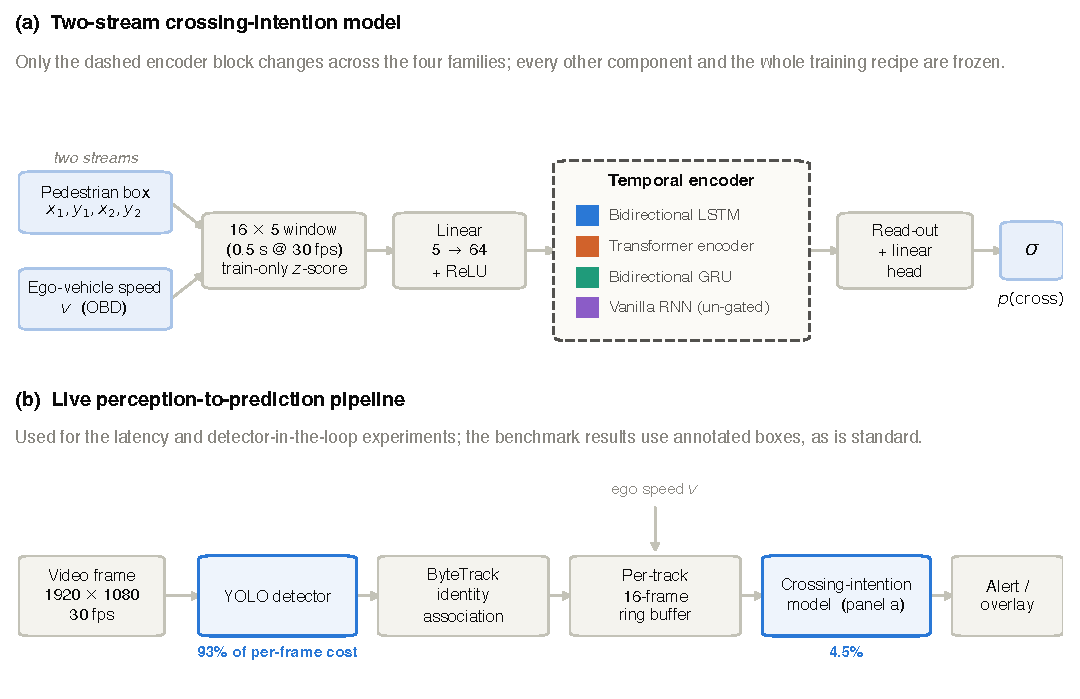
\includegraphics[width=\textwidth]{figures/fig2_system.pdf}
\caption{The two-stream crossing-intention model and the pipeline it runs inside. (\textbf{a}) A sixteen-frame window of pedestrian bounding-box coordinates and ego-vehicle speed is projected, passed through a temporal encoder, and read out to a single crossing probability; only the dashed encoder block differs across the four model families compared in this paper. (\textbf{b}) In deployment the same model runs behind a YOLO26-M detector and a ByteTrack tracker, annotated here with each stage's measured share of the per-frame cost on an Apple M4.\label{fig:system}}
\end{figure}

\subsection{The PIE Dataset and Splits}

The Pedestrian Intention Estimation (PIE) dataset~\citep{rasouli2019pie} provides over six hours of driving recorded in downtown Toronto at $1920 \times 1080$ and 30 fps, divided into six recording sets. Each pedestrian carries per-frame bounding boxes, a per-frame \texttt{cross} state, a binary crossing label and a \texttt{crossing\_point} event frame, with on-board diagnostics supplying vehicle speed synchronised to the video. Parsing yields 582,376 frame-level rows covering 1,374 pedestrians once those labelled \texttt{crossing\_label}~$=-1$ are dropped.

We split by recording set rather than at random: set01, set02 and set04 train, set05 and set06 validate, set03 tests. Recording sets partition the videos, so no pedestrian, scene or video appears in more than one split, which a random split over windows would not guarantee. Two conventions circulate under the name of the standard protocol. The benchmark of Kotseruba et al.~\citep{kotseruba2021benchmark} trains on set01, set02 and set06 and validates on set04 and set05, while the dataset's own toolkit defaults to the assignment we use. Set03 is the test set under both, so published test numbers remain broadly commensurable, and we note the difference wherever we tabulate other work.

The training split contains 1,366 negative and 812 positive windows, a ratio of 1.682. That ratio is the positive-class weight in the training loss, computed after the split from training data alone; had it been computed over the pooled data it would have been 1.977, a value that would have seen the validation and test class distributions. Weighting is not the only option: Buda et al.~\citep{buda2018systematic} found oversampling dominant across their settings, though at imbalance ratios far more severe than 1.682:1. Rather than assume their finding transfers, we swept the weight over $\{1.0, 1.3, 1.682, 2.1, 2.5\}$ on validation data for two of the four families and confirmed the anchor value (Section~\ref{sec:settings}).

\subsection{Temporal Leakage and the Leakage-Free Protocol}

A model asked to predict whether a pedestrian will cross must not be shown the crossing. The widely used extraction anchors each window at the last annotated frame minus a time-to-event offset, which constrains nothing about where the crossing onset falls. Leakage of this kind is a recognised failure mode, and detecting it means checking the temporal relationship between features and target event directly~\citep{kaufman2012leakage}. The dataset's authors have separately noted that intention clips terminate at a \texttt{critical\_point} while action samples are drawn at one to three seconds time-to-event, so the two tasks do not share an anchor~\citep{rasouli2024diving}; what has not been reported is how often the observation window overlaps the event it is supposed to precede.

We measured it. PIE annotates a per-frame \texttt{cross} state that the common parser discards; recovering it turns the question into a count. Of 570 crossing sequences under the track-end anchor, 387 (67.9\%) contain at least one frame in which the pedestrian is already crossing, and 369 (64.7\%) are crossing in all sixteen observed frames, so for those sequences the task has become detection. Only 183 (32.1\%) have a clean window. The median gap between the end of the window and crossing onset is $+182$ frames, on the wrong side of zero. A second symptom: the bounding box at the anchor frame alone separates the classes, with rank-biserial correlations of $+0.65$ for box area, $+0.63$ for height and $+0.49$ for the bottom edge, so a model can read screen geometry instead of motion.

The fix uses an event the dataset already provides. We anchor at \texttt{crossing\_point}, truncate the contiguous track segment containing it at that frame inclusive, and slide 16-frame windows at 50\% overlap, keeping only windows whose last observed frame falls 30 to 60 frames before the event. Pedestrians whose truncated track is shorter than the window plus the minimum look-ahead are excluded, costing 107 of 1,374 pedestrians (7.8\%). Figure~\ref{fig:protocol} contrasts the two rules.

\begin{figure}[H]
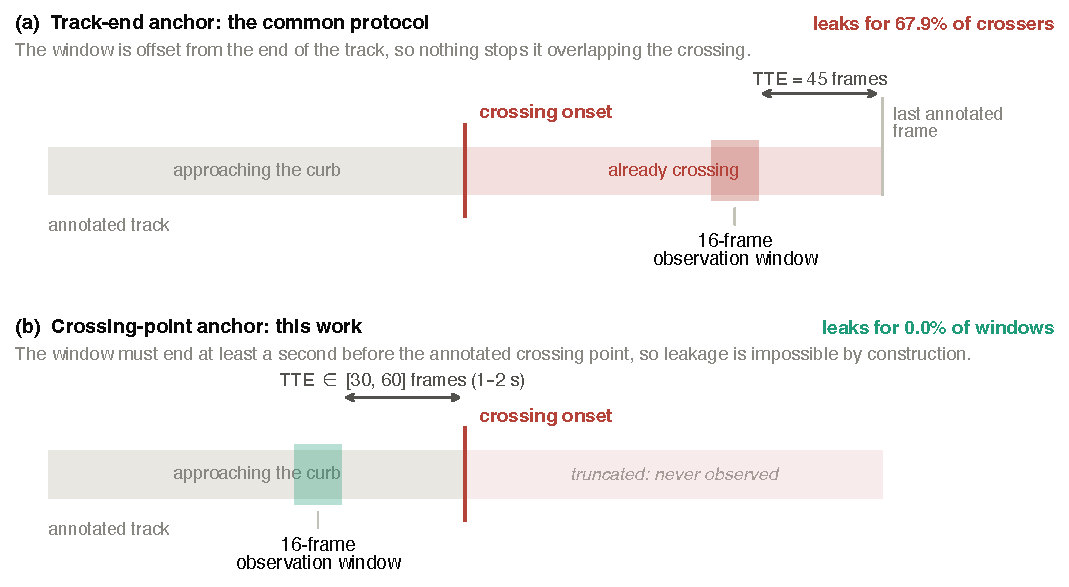
\includegraphics[width=\textwidth]{figures/fig3_protocol.pdf}
\caption{Where the sixteen-frame observation window falls under each anchoring rule on PIE. (\textbf{a}) Anchoring at the end of the annotated track places no constraint on the crossing onset, so the window may overlap the crossing it is meant to predict; this occurs for 67.9\% of crossing sequences. (\textbf{b}) Anchoring at the dataset's own \texttt{crossing\_point} event and requiring the last observed frame to fall 30 to 60 frames earlier makes that overlap impossible by construction, verified at 0 of 4,906 windows.\label{fig:protocol}}
\end{figure}

Two properties make the result leak-free by construction rather than by inspection. First, \texttt{crossing\_point} coincides with the first frame labelled as crossing for 516 of 519 crossers (99.4\%) and never precedes it, so truncating there cannot leave crossing frames behind. Second, the 30-frame minimum look-ahead separates the last observed frame from the event by at least one second. Re-running the audit on the rebuilt data confirms the construction: 0 of 4,906 windows contain a crossing frame, and the median gap moves to $-44$ frames. The geometric shortcut collapses with it, to $+0.25$, $+0.21$ and $+0.09$, all below the conventional threshold for a medium effect. Table~\ref{tab:protocol} reports both protocols side by side.

Two consequences follow. The re-extraction is 3.5 times larger, because sliding windows over truncated tracks recovers samples that one-window-per-track discards, and the best validation checkpoint moves from epoch 3 to epoch 17, the signature of a harder learning problem. Removing the leakage costs little in headline terms, which is the point: the old protocol produced roughly the right number for partly the wrong reason.

Because a larger sample invites the suspicion of an easier one, we checked four ways. Scoring per window gives AUC 0.9131; averaging predictions per pedestrian gives 0.9143, so window overlap does not inflate the estimate; restricting to tracks long enough for the stricter benchmark filter gives 0.9194; and the short tracks our looser floor admits score 0.8634. The additional data is harder than the data it joins.

\begin{table}[H]
\caption{Track-end versus \texttt{crossing\_point} anchoring on PIE. Re-anchoring removes all window leakage and grows the usable sample 3.5-fold. Window counts are given as total (train/validation/test); the class weight is the positive-class weight in the training loss, equal to the training split's negative-to-positive ratio; rank-biserial correlations measure how well the bounding box at the last observed frame alone separates crossers from non-crossers.\label{tab:protocol}}
\begin{tabularx}{\textwidth}{lCC}
\toprule
\textbf{Property} & \textbf{Track-end anchor} & \textbf{\texttt{crossing\_point} anchor}\\
\midrule
Anchor rule & last annotated frame $-$ TTE & \texttt{crossing\_point}, TTE $\in [30,60]$\\
Sampling & one window per segment & 50\% overlap, stride 8\\
Windows (train/val/test) & 1389 (616/186/587) & 4906 (2178/634/2094)\\
Positive rate & 41.0\% & 33.6\%\\
Crossers observed mid-crossing & 387/570 (67.9\%) & 0/1648 (0.0\%)\\
Windows containing a crossing frame & 387/1389 (27.9\%) & 0/4906 (0.000\%)\\
Box area, rank-biserial & $+0.65$ & $+0.25$\\
Box height, rank-biserial & $+0.63$ & $+0.21$\\
Box bottom edge, rank-biserial & $+0.49$ & $+0.09$\\
Training class weight & 1.44 & 1.682\\
Best validation epoch & 3 & 17\\
\bottomrule
\end{tabularx}
\end{table}

\subsection{Features and Preprocessing}

Each window is sixteen frames, 0.53 s at 30 fps, of a five-dimensional vector: the four bounding-box coordinates and the ego-vehicle speed. Coordinates stay in raw pixels rather than being divided by the image dimensions. A per-feature $z$-score removes any fixed scale factor, so the choice does not affect what the model sees, and raw pixels keep the inference contract identical to the annotation format, with no implicit dependence on a resolution constant. The standardisation statistics come from the training split alone and are applied unchanged to validation and test, because fitting any preprocessing step on data used for evaluation is itself leakage~\citep{kaufman2012leakage}. Unless a validation-tuned threshold is stated, decisions use 0.5 on the sigmoid output.

\subsection{Model Architectures}

All four families share one wrapper: a linear projection of the five inputs to 64 dimensions with a ReLU, a temporal encoder, a read-out from the pooled or final step, and a linear layer to a single logit. Only the encoder differs, so each comparison isolates one design choice.

The bidirectional LSTM~\citep{hochreiter1997lstm,schuster1997bilstm} is the reference: two layers, hidden size 128, dropout 0.3, 594,561 parameters. Swapping \texttt{nn.LSTM} for \texttt{nn.GRU}~\citep{cho2014gru,chung2014gru} gives the gated recurrent twin at 446,081 parameters, isolating which gated cell is used; swapping it for a bidirectional tanh \texttt{nn.RNN}~\citep{elman1990rnn,rumelhart1986backprop} removes gating altogether at 149,121 parameters, isolating gating itself. The three form a ladder: if the LSTM's gates carry the task, removing them should cost something measurable. The fourth family is a pre-layer-norm Transformer encoder~\citep{vaswani2017attention,xiong2020prelayernorm}: the searched configuration uses four heads, width 128, feed-forward width 512, four layers, last-token pooling and sinusoidal positional encoding, at 794,241 parameters, and the un-searched control uses feed-forward width 256, two layers, a classification token and learned positional encoding, at 268,417 parameters. An ablation replaces the LSTM's final-step read-out with additive attention~\citep{bahdanau2015attention}, at 611,265 parameters.

Capacity has to be equalised somehow, and the two available conventions disagree. Chung et al.~\citep{chung2014gru} chose each model's size so that all cells had approximately the same parameter count. We instead hold the recurrent width fixed at 128 and let the parameter count follow the cell, because a cell swap is the manipulation under test and re-widening each cell would confound it with a capacity change. The consequence works against our own conclusion: at matched width the gated LSTM has 594,561 parameters against the un-gated RNN's 149,121, so the gated cell holds a fourfold capacity advantage, and a tie is reached by the smaller model from behind. Parameter counts appear in every results table so either reading stays available, and a second design lets each family choose its own width under an identical search budget (Section~\ref{sec:settings}).

Every crossing-intention model here is trained from scratch. The only pretrained component in this work is the object detector in the live pipeline, which enters no tabulated comparison.

\subsection{Metric Hierarchy, Evaluation, and Statistical Procedure}

We report F1 first, then accuracy, then ROC-AUC and PR-AUC. The literature supports part of this ordering and not all of it: accuracy is a poor summary under class imbalance, and precision-recall analysis is more informative than ROC analysis when the classes are skewed~\citep{davis2006precision,saito2015precision}. It does not establish F1 as the primary metric, and we do not claim that it does. The ordering is a reporting choice appropriate to an imbalanced, safety-critical decision, and the threshold-free measures corroborate it without carrying the headline.

Model selection touches validation data only. A tuned decision threshold is fitted on the validation split, because selection performed on evaluation data biases the reported estimate~\citep{cawley2010overfitting}, and the test set is scored once per experiment with every choice already fixed.

Two properties of the test set govern the statistics. Its 2,094 windows come from 541 pedestrian tracks at 50\% overlap, so windows are not independent; we resample whole pedestrians, the standard treatment for one-way clustered data~\citep{fieldwelsh2007}, and quote those intervals wherever a confidence interval appears. Model contrasts use paired bootstrap resampling, scoring both models on identical resamples so the interval describes the difference and not each model's separate variability~\citep{koehn2004significance}. All bootstraps use 10,000 resamples. We report two statistics that are never mixed in one sentence: the per-seed mean over five seeds, which is what other papers report, and the five-seed probability ensemble, which is one deployable predictor and scores slightly higher.

\subsection{Live Perception-to-Prediction Pipeline}

To measure the model where its inputs are estimated rather than annotated, we run it behind a detector and a tracker. Frames go to a YOLO26-M person detector (Ultralytics YOLO, \url{https://github.com/ultralytics/ultralytics}), detections to ByteTrack~\citep{zhang2022bytetrack} for identity association, and each track keeps a rolling 16-frame buffer of box coordinates and ego speed, standardised with the training statistics. The reader preserves absolute PIE frame numbers so the speed lookup stays aligned with the video. Per frame the detector costs 33.7 ms, association about 1.0 ms and the intention model 1.647 ms, giving 36.4 ms and 27.5 frames per second; the prediction model is 4.5\% of that budget. Section~\ref{sec:results} reports what happens to the predictions when the boxes come from the detector instead of the annotations.

\section{Experimental Settings}
\label{sec:settings}

Training, the statistical analysis, the recurrent searches and all timing ran on an Apple M4 with ten CPU cores and 16 GB of unified memory under macOS 26.5. The larger Transformer search and the observation-length sweeps used a Kaggle NVIDIA T4. Every configuration appearing in a table was then retrained locally through the same engine, with inference parity between the two environments verified at about $10^{-6}$, so no tabled number depends on which machine produced it. The software stack is Python 3.13.5, PyTorch 2.12.0~\citep{paszke2019pytorch}, NumPy 2.4.6, SciPy 1.17.1 and scikit-learn 1.9.0; the live pipeline adds Ultralytics 8.4.68 with a YOLO26-M detector and the bundled ByteTrack implementation.

One measured property of the hardware decides where recurrent runs execute. Training \texttt{nn.LSTM} on Apple's MPS backend is process-history-dependent: the same configuration and seed give different results according to what ran earlier in the same process. CPU training is bit-reproducible and context-free, and Transformer training does not show the effect. Recurrent runs needing exact reproduction therefore execute on CPU, where the cross-family replication was done.

The training recipe is frozen and shared: binary cross-entropy with a positive-class weight of 1.682 in the training gradient only, Adam~\citep{kingma2015adam} with weight decay $10^{-5}$, batch size 32, at most 100 epochs, early stopping with patience 15 on validation AUC, and a plateau scheduler halving the learning rate after five epochs without improvement. Each configuration is trained with five seeds, $[42, 0, 1, 2, 3]$. The checkpoint kept is the best validation epoch under whichever rule is in force, validation AUC or validation F1 with ties broken by accuracy then AUC, never the last epoch. Set03 is evaluated once per experiment on the selected checkpoint. One configuration departs from the shared recipe: the tuned Transformer's F1 arm uses a positive-class weight of 2.5, chosen by its own validation sweep over $\{1.0, 1.3, 1.682, 2.1, 2.5\}$. Every other model uses 1.682, which the same sweep confirmed for the recurrent families.

Search budgets were fixed in advance. The three recurrent families received an identical grid over learning rate $\{10^{-3}, 5\times10^{-4}, 10^{-4}\}$, dropout $\{0.2, 0.3, 0.5\}$, hidden size $\{64, 128, 256\}$ and depth $\{1, 2\}$: 54 nominal cells collapsing to 36 distinct configurations, since inter-layer dropout is inert at depth 1. Selection ran in three stages: all 36 at one seed ranked by validation AUC, then the top five and the hand-set baseline across all five seeds with the winner taken as the best five-seed mean, and only then the winner and baseline on test. The single-seed leader was not the five-seed winner, which is what the second stage is for. The Transformer received 78 configurations because it has more architectural freedom than a cell swap allows: 36 architectures over width, depth, pooling and positional encoding, 36 recipes on the best of them, six transfer checks on the next two architectures, and a final stage over the top five plus a pre-registered default. No stage of any search evaluated the test set.

The comparison is then run twice, for a documented reason: an architecture comparison measures tuning effort as much as architecture. Melis et al.~\citep{melis2018sota} re-evaluated language-model architectures under large-scale tuning and found a properly regularised LSTM beating the newer models it had supposedly lost to, attributing the earlier result to differing code bases and compute. Lucic et al.~\citep{lucic2018gans} found the same for generative adversarial networks: most models reach similar scores given enough hyperparameter optimisation, so gains often come from budget instead of algorithmic change. Greff et al.~\citep{greff2017odyssey} tuned each of eight LSTM variants separately across 5,400 runs and found none significantly better than the standard cell.

In the tuned design, each family therefore selects its own configuration under an identical budget. The apparent alternative, imposing one family's recipe on all four, sounds fairer and is not: it relocates the bias onto whichever family that recipe happens to suit. Our own searches show it. The un-gated RNN selected a learning rate of $10^{-4}$, an order of magnitude below the LSTM's $10^{-3}$. Training the RNN at the LSTM's rate would not have measured the cell; it would have measured how well an un-gated cell tolerates a learning rate chosen for a gated one.

The matched design answers the complementary question and carries a problem of its own. Holding the recurrent width at 128 keeps the cell swap as the only manipulation, but capacity does not follow width evenly across cells: at width 128 an LSTM carries four gate matrices where the un-gated cell carries one and the GRU three, giving 594,561, 149,121 and 446,081 parameters. Chung et al.~\citep{chung2014gru} handled this the other way, sizing each model so all cells had approximately equal parameter counts. We match width because a cell swap requires it, and report parameter counts in every table so either reading stays available. The asymmetry works against our own conclusion: the gated cells hold the capacity advantage, so any tie is reached by the smaller model.

Five seeds is too small a sample for a well-powered significance test across training runs~\citep{bouthillier2021variance,reimers2017reporting}. Seed spread is therefore reported descriptively, and every comparative claim rests on the bootstrap procedures of Section~\ref{sec:methods}, where the resampling unit is 541 test pedestrians and not five runs. Table~\ref{tab:hparams} gives the configuration each search selected.

\begin{table}[H]
\caption{The configuration selected by each family's own search under the F1-first rule, with the parameter count of the selected model. Everything not listed is identical across families: batch size 32, at most 100 epochs, early stopping with patience 15, train-only $z$-score standardisation, Adam with weight decay $10^{-5}$, and five seeds. Width is the recurrent hidden size, the read-out being twice this for a bidirectional cell, or the Transformer's model and feed-forward dimensions. The decision threshold $\tau$ is tuned on validation data only. The Transformer's class weight of 2.5 is the single departure from the shared value of 1.682, selected by its own validation sweep.\label{tab:hparams}}
\begin{tabularx}{\textwidth}{lCCCCCCC}
\toprule
\textbf{Family} & \textbf{Width} & \textbf{Layers} & \textbf{Dropout} & \textbf{LR} & \textbf{Weight} & \textbf{$\tau$} & \textbf{Params}\\
\midrule
LSTM & 256 & 2 & 0.3 & $10^{-3}$ & 1.682 & 0.52 & 2,237,313\\
Transformer & 128/512 & 4 & 0.1 & $10^{-3}$ & 2.5 & 0.65 & 794,241\\
GRU & 256 & 2 & 0.3 & $5\times10^{-4}$ & 1.682 & 0.53 & 1,678,209\\
RNN & 256 & 2 & 0.2 & $10^{-4}$ & 1.682 & 0.53 & 560,001\\
\bottomrule
\end{tabularx}

\noindent{\footnotesize The Transformer uses four attention heads, last-token pooling and sinusoidal positional encoding; the recurrent families are bidirectional and read out from the final step.}
\end{table}

\section{Results}
\label{sec:results}

\subsection{The Temporal-Leakage Audit}

Under the track-end anchor, 387 of 570 crossing sequences (67.9\%) contain at least one frame in which the pedestrian is already crossing, and 369 (64.7\%) are crossing throughout the observation window. Figure~\ref{fig:leakage}a shows the distribution. The median gap between the last observed frame and crossing onset is $+182$ frames, so the typical positive sequence reaches almost six seconds into the event it is meant to anticipate. The static shortcut in Figure~\ref{fig:leakage}b is the second symptom: the box at the anchor frame separates the classes on its own, at rank-biserial $+0.65$ for area, $+0.63$ for height and $+0.49$ for the bottom edge.

Re-anchoring at \texttt{crossing\_point} removes both. No window among the 4,906 contains a crossing frame, and the geometric correlations fall to $+0.25$, $+0.21$ and $+0.09$. That the shortcut collapses alongside the leakage indicates the two were connected: part of what made crossers look geometrically distinctive was that they were being observed mid-crossing, close to the camera and low in the frame.

\begin{figure}[H]
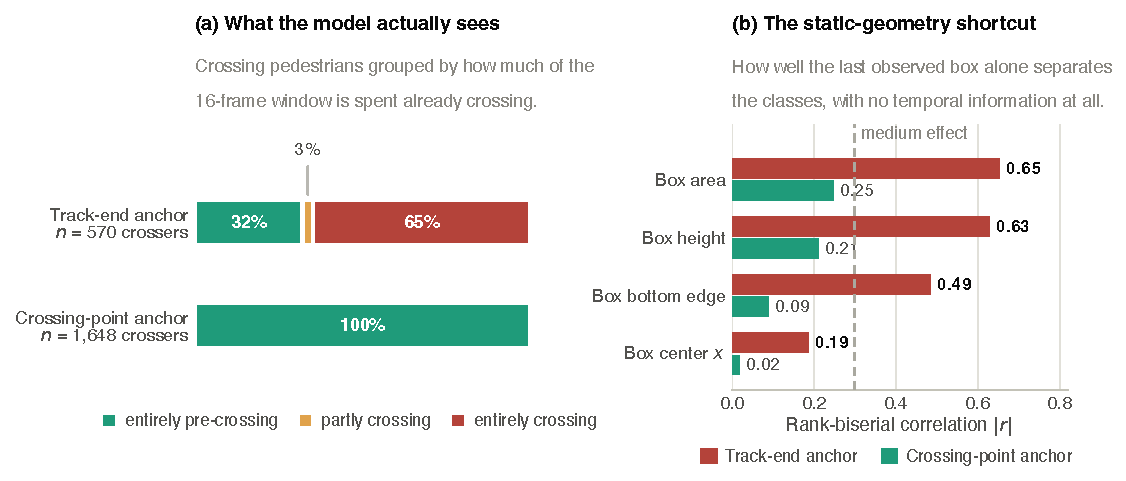
\includegraphics[width=\textwidth]{figures/fig4_leakage.pdf}
\caption{The temporal-leakage audit on PIE, computed from the dataset's own per-frame \texttt{cross} annotations. (\textbf{a}) Crossing sequences grouped by how many of the sixteen observed frames already show the pedestrian crossing, under the track-end anchor and under \texttt{crossing\_point} anchoring. (\textbf{b}) How well the bounding box at the last observed frame alone separates crossers from non-crossers under each rule, as rank-biserial correlation; values below 0.3 indicate no usable static shortcut.\label{fig:leakage}}
\end{figure}

\subsection{Main Result}

On the leakage-free protocol the reference bidirectional LSTM reaches F1 $0.828 \pm 0.012$, accuracy $0.883 \pm 0.009$ and ROC-AUC $0.932 \pm 0.011$ over five seeds, with PR-AUC 0.876 against a base rate of 32.5\%. The bootstrap 95\% confidence interval on AUC is $[0.92, 0.95]$ resampling windows and $[0.92, 0.96]$ resampling the 541 test pedestrians as clusters. The best F1 obtained by any model in this paper is $0.852 \pm 0.012$, from the tuned un-gated RNN.

The AUC before the leakage was removed was 0.931. After removal it is 0.932. This near-identity is the finding, not a reassurance about it: a protocol that showed roughly two thirds of its positive windows to the model mid-crossing produced approximately the same headline number as one that shows none, which means the headline number was never diagnostic of whether the task was prediction or detection. What does change is the shape of training. The best validation epoch moves from 3 to 17, and the geometric shortcut disappears.

The obvious alternative explanation is that the new protocol is simply easier, since it yields 3.5 times more data. Four checks rule that out. Scoring per window gives AUC 0.9131 and averaging predictions within each pedestrian gives 0.9143, so the 50\% window overlap inflates nothing. Restricting to tracks long enough to pass the stricter benchmark length filter gives 0.9194, and the short tracks admitted by our looser floor score 0.8634 on their own. The additional windows are harder than the ones they join.

\subsection{Does the Architecture Matter?}

Table~\ref{tab:families} reports all four families under both designs, with the two ablations. Under the tuned design the four F1 values span 0.844 to 0.852, a range of 0.008 against per-seed standard deviations of 0.008 to 0.017.

Every cross-family contrast on F1 is a tie. Against the tuned LSTM, the GRU gives $\Delta$F1 $+0.0071$ with a 95\% pedestrian-cluster interval of $[-0.0043, +0.0187]$, the un-gated RNN $+0.0033$ $[-0.0083, +0.0150]$, and the Transformer $+0.0008$ $[-0.0124, +0.0142]$ at $p = 0.762$. The RNN against the GRU gives $-0.0038$ $[-0.0117, +0.0039]$. Every interval spans zero. Figure~\ref{fig:forest}a shows them together. We report these as ties and not as a win for the RNN, whose point estimate is nominally highest, because the intervals do not license an ordering.

A tie is only informative if the test can detect a difference, and on this data it can. The same paired bootstrap on the same windows finds the F1-optimised LSTM better than its own AUC-selected baseline by $+0.0187$ $[+0.0073, +0.0300]$, which survives pedestrian-cluster resampling at $[+0.0043, +0.0349]$. It finds the searched Transformer better than the AUC-selected LSTM on AUC by $+0.0135$ $[+0.0097, +0.0174]$. And it finds the ego-speed ablation separated from everything by a margin no interval comes near. The procedure separates models when models differ.

On AUC the searched Transformer does have an advantage: $0.950 \pm 0.003$ against the LSTM's $0.932$, a paired-bootstrap $\Delta$ of $+0.0135$ $[+0.0097, +0.0174]$, with a five-seed paired $t$-test at $p = 0.025$. The location of that advantage is the more useful result. Running the same Transformer architecture with the LSTM's own un-searched recipe gives $\Delta$AUC $+0.0005$ $[-0.0034, +0.0043]$, a tie. Attention does not beat recurrence on this signal; a search budget spent on architecture and recipe found a better configuration, and the configuration it found differs from the default in depth, pooling and positional encoding. The un-gated RNN closes the same gap when given the same treatment, reaching $\Delta$AUC $-0.0013$ $[-0.0041, +0.0015]$ against the searched Transformer, while the GRU does not, at $-0.0070$ $[-0.0101, -0.0038]$.

\begin{table}[H]
\caption{All four families on the leakage-free PIE test set (set03, 2,094 windows, 32.5\% positive) under both comparison designs, with two ablations of the reference model. Values are per-seed means over five seeds with standard deviations where relevant; F1 leads because it is the primary metric. In the matched design the recurrent families share width 128 so that only the cell changes. ($\dagger$) Attention has no hidden-size equivalent, so the matched Transformer is the un-searched default configuration, and it is the one row selected on validation F1 rather than validation AUC; selecting it on validation AUC instead gives AUC 0.934. No cross-family difference in either design is significant on F1 (Figure~\ref{fig:forest}a).\label{tab:families}}
\begin{tabularx}{\textwidth}{llCCCC}
\toprule
\textbf{Design} & \textbf{Family} & \textbf{Params} & \textbf{F1} & \textbf{Acc} & \textbf{AUC}\\
\midrule
\multirow{4}{*}{Matched} & LSTM & 594,561 & 0.828 & 0.883 & 0.932\\
 & GRU & 446,081 & 0.840 & 0.898 & 0.933\\
 & RNN & 149,121 & 0.836 & 0.889 & 0.942\\
 & Transformer \textsuperscript{$\dagger$} & 268,417 & 0.821 & 0.878 & 0.942\\
\midrule
\multirow{4}{*}{Tuned} & LSTM & 2,237,313 & 0.844 & 0.897 & 0.940\\
 & Transformer & 794,241 & 0.847 & 0.896 & 0.947\\
 & GRU & 1,678,209 & 0.849 & 0.901 & 0.941\\
 & RNN & 560,001 & \textbf{0.852} & 0.902 & 0.948\\
\midrule
\multirow{2}{*}{Ablation} & LSTM, box only & 594,497 & 0.551 & 0.744 & 0.753\\
 & LSTM $+$ attention & 611,265 & 0.821 & 0.879 & 0.925\\
\bottomrule
\end{tabularx}
\end{table}

\begin{figure}[H]
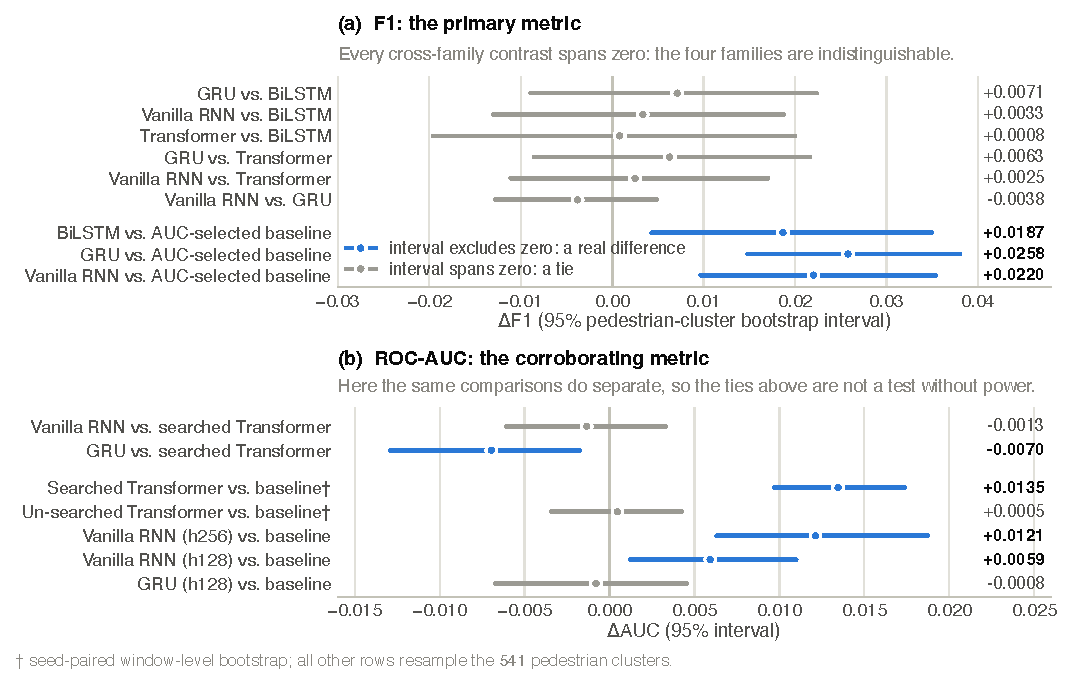
\includegraphics[width=\textwidth]{figures/fig6_forest_compact.pdf}
\caption{Paired contrasts computed on identical resamples of the test set, with 95\% pedestrian-cluster bootstrap intervals over the 541 test pedestrians. (\textbf{a}) On F1, every cross-family contrast spans zero, while the lower group shows the same procedure detecting effects that are real. (\textbf{b}) On ROC-AUC the models do separate, with matched-configuration contrasts shown beside tuned ones.\label{fig:forest}}
\end{figure}

\subsection{Comparison with Published Baselines}

Table~\ref{tab:baselines} places our models against published PIE results. Two facts about it, stated rather than ranked. The highest F1 in the table is PIP-Net's 0.88, obtained at a 0.5 s prediction horizon with seven input streams. The highest F1 among methods evaluated at a horizon comparable to ours is PedFormer's 0.87, with our four families 0.02 to 0.03 below it using two streams.

The horizon column exists because horizon dominates this comparison, and our own ablation is the evidence. On a fixed cohort of the same 493 test pedestrians, AUC falls from 0.961 at a 1.0 s horizon to 0.919 at 2.0 s (Section~\ref{sec:horizon}). A method evaluated at 0.5 s is answering an easier question than one evaluated at 1--2 s, so cross-paper differences of the size seen in this table are within the range that horizon alone can produce.

Three further caveats belong with the table. Our protocol is leakage-free and the tabulated protocols are not, so the comparison is indicative and not a like-for-like leaderboard. The evaluation code of the reference benchmark computes ROC-AUC on thresholded predictions instead of continuous scores, so not every tabulated AUC is the same statistic as ours. And PedCMT~\citep{chen2024pedcmt}, which reaches comparable performance on bounding boxes and ego-speed alone, is discussed in Section~\ref{sec:related-work} but not tabulated: no open-access version of its results exists, and its released code uses a random 70/15/15 split, so its numbers are not standard-protocol comparable.

\begin{table}[H]
\caption{Crossing prediction on PIE. Baseline figures are as reported by the cited sources, verified against each method's own paper where an accessible version exists; entries marked ($\ddagger$) were available only through another paper's comparison table. Our rows are per-seed means over five seeds at threshold 0.5. Our protocol is leakage-free and therefore not strictly identical to the protocols behind the other rows, so this table is indicative rather than a like-for-like leaderboard. Horizon is the prediction horizon each method evaluated at; ``n.r.'' marks methods whose horizon we could not verify from a primary source.\label{tab:baselines}}
\begin{adjustwidth}{-\extralength}{0cm}
\begin{tabularx}{\fulllength}{lcccclL}
\toprule
\textbf{Method} & \textbf{Acc} & \textbf{AUC} & \textbf{F1} & \textbf{Horizon} & \textbf{Streams} & \textbf{Modalities}\\
\midrule
PCPA~\citep{kotseruba2021benchmark} & 0.87 & 0.86 & 0.77 & 1--2 s & 4 & box, pose, context, speed\\
Pedestrian Graph$+$~\citep{cadena2022pedgraph} $^\ddagger$ & 0.89 & 0.90 & 0.81 & n.r. & 2--3 & pose graph, ego\\
IntFormer~\citep{lorenzo2021intformer} & 0.89 & 0.92 & 0.81 & 1--2 s & 4 & box, crops, pose, speed\\
PIT~\citep{zhou2023pit} $^\ddagger$ & 0.91 & 0.92 & 0.82 & 1--2 s & 5 & multimodal\\
BiPed~\citep{rasouli2021biped} & 0.91 & 0.90 & 0.85 & 1--2 s & 4 & multimodal multitask\\
PedFormer~\citep{rasouli2023pedformer} & 0.93 & 0.90 & 0.87 & 1--2 s & 4 & multimodal multitask\\
GTransPDM~\citep{xie2025gtranspdm} & 0.90 & 0.87 & 0.82 & 1--2 s & 3 & box, pose, ego\\
GTransPDM, no pose~\citep{xie2025gtranspdm} & 0.92 & 0.90 & 0.86 & 1--2 s & 2 & box, ego motion\\
MFT~\citep{li2025mft} & 0.90 & 0.94 & 0.83 & 1--2 s & 4 & numerical context\\
PIP-Net~\citep{azarmi2025pipnet} & 0.92 & 0.94 & 0.88 & 0.5 s & 7 & box, pose, RGB, flow, semantics, depth, speed\\
\midrule
LSTM (ours) & 0.897 & 0.940 & 0.844 & 1--2 s & 2 & box, ego speed\\
Transformer (ours) & 0.896 & 0.947 & 0.847 & 1--2 s & 2 & box, ego speed\\
GRU (ours) & 0.901 & 0.941 & 0.849 & 1--2 s & 2 & box, ego speed\\
RNN (ours) & 0.902 & 0.948 & 0.852 & 1--2 s & 2 & box, ego speed\\
\bottomrule
\end{tabularx}
\end{adjustwidth}
\end{table}

\subsection{Which Input Carries the Signal?}

Removing ego-vehicle speed from an otherwise identical LSTM collapses it: F1 falls from 0.828 to 0.551, accuracy from 0.883 to 0.744 and AUC from 0.932 to 0.753. The bootstrap intervals do not approach each other, the box-only model topping out near 0.78 where the two-stream model starts at 0.92. Losing one of two inputs costs 0.18 AUC, which identifies ego speed as the dominant stream. The finding is confirmatory. A contextual permutation analysis reached it independently, and warned that reliance on ego speed may introduce a driver-side bias in yielding scenarios~\citep{azarmi2024featureimportance}.

Adding capacity to the temporal model does nothing comparable. Replacing the LSTM's final-step read-out with additive attention moves AUC from 0.932 to 0.925 and F1 from 0.828 to 0.821, both within seed noise.

\subsection{Prediction Horizon and Observation Length}
\label{sec:horizon}

Horizon matters and window length does not. On the matched cohort of 493 test pedestrians eligible at every horizon, AUC falls from $0.961$ at 1.0 s to $0.946$ at 1.5 s and $0.919$ at 2.0 s, with every pairwise paired $t$-test at $p \le 0.004$ and Kruskal--Wallis $p = 0.002$. Restricting all three conditions to a common cohort changes the numbers by at most 0.002, so the decline is not an artefact of which pedestrians qualify at each horizon. On the unmatched sampling the same pattern holds at $0.960 / 0.948 / 0.919$, $p \le 0.008$.

This overturns a conclusion we previously drew ourselves. On the leaky protocol the model appeared insensitive to horizon, which we now read as a symptom and not a finding: a model detecting an in-progress crossing is indifferent to the nominal distance to an event it is already observing. Once the event is genuinely in the future, performance degrades with distance from it, as it should.

Observation length behaves the other way. At 8, 16 and 30 frames, AUC is $0.931$, $0.933$ and $0.937$; no pairwise test reaches significance, the smallest $p$ being 0.21, and the between-condition spread of 0.0058 is smaller than the average within-condition seed standard deviation of 0.0073. Extending to 32 and 64 frames lowers F1 for all four families. That sweep is not a matched cohort: a longer window requires a longer pre-crossing track, so the usable test set shrinks from 2,094 windows to 1,009 and then 458, and the cohort shifts with it. Read within a window and not across windows, one result stands out. At 64 frames the un-gated RNN alone falls behind, losing 0.050 F1 against its own 16-frame result where the gated cells lose 0.026 to 0.028. Per-seed intervals still overlap, so this is directional, but it is the direction theory predicts and it bounds the equivalence result: gating is redundant over half a second and begins to matter by two.

\subsection{Cross-Set Generalization, Capacity, and Latency}

Leave-one-set-out over all six recording sets gives AUC $0.928 \pm 0.041$, or $0.915 \pm 0.029$ excluding the 47-window set05 fold, which is too small to interpret. The fold that holds out set03, our fixed test set, scores 0.931, sitting at the fold mean and not above it, so set03 is not an unusually easy partition. The other families behave similarly, at 0.946 for the GRU, 0.939 for the Transformer and 0.937 for the RNN.

Capacity is not the binding constraint. Hidden sizes 64, 128 and 256 give AUC $0.927$, $0.933$ and $0.938$, with 256 against 128 not significant at $p = 0.338$ despite 3.8 times the parameters; depths 1, 2 and 3 give $0.930$, $0.932$ and $0.931$, a spread far inside seed noise. The 36-configuration grid search beat the hand-set baseline on test by $+0.0006$ at $p = 0.914$, which is to say it confirmed it.

All four families are far inside a real-time budget on CPU at batch 1: 0.316 ms per window for the RNN, 0.459 for the Transformer, 0.575 for the LSTM and 0.721 for the GRU, or 46 to 105 times inside the 33.3 ms of a 30 fps frame. Latency does not discriminate between these models. In the full pipeline the detector accounts for 92.7\% of per-frame cost and the intention model 4.5\%, giving 27.5 frames per second end to end.

\subsection{Detector-in-the-Loop Robustness}

Replacing annotated boxes with detected ones costs little. Across 311 windows from 98 pedestrians in two test clips, with mean IoU 0.750 between detected and annotated boxes, per-window AUC falls from 0.962 to 0.953 and per-pedestrian AUC from 0.958 to 0.948, and the thresholded decision flips in 10 of 311 windows (3\%).

Two limits on that number. It is a lower bound on deployed degradation, because detections are matched to annotations by best overlap, which isolates box-quality noise and removes the association errors a deployed system would make. The pipeline's weak points are in perception, not prediction. The detector covers 88\% of pedestrians, so roughly one in eight is never tracked well enough to predict for at all, and a single ByteTrack identity covers a mean of 39\% of a pedestrian's frames, with 59\% of windows carrying a competing identity. Deployment would need re-identification before it needed a better intention model.

\subsection{Qualitative Behaviour}

Figure~\ref{fig:qualitative} shows the pipeline running on two test clips with boxes from the detector and tracker, using the five-seed LSTM ensemble at its validation-tuned threshold of 0.516. In the first panel a pedestrian is flagged at $p = 0.71$ about 1.5 s before stepping off the kerb; in the second a worker standing at a kerb beside a crosswalk is correctly left at $p = 0.31$. Both panels were selected to illustrate behaviour, not to sample it, so the quantitative failure rates in the preceding subsections are the representative numbers. Across all 439 windows in these two clips the ensemble gives 134 true positives, 16 false positives, 19 false negatives and 270 true negatives, an accuracy of 0.920 and F1 of 0.884. Faces were irreversibly blurred before publication.

\begin{figure}[H]
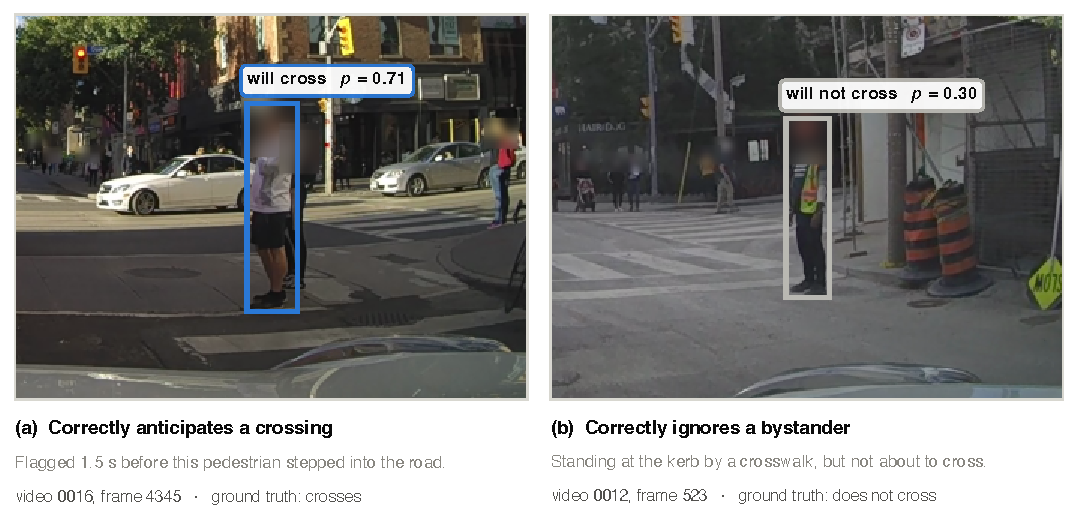
\includegraphics[width=\textwidth]{figures/fig9_qualitative.pdf}
\caption{The detection-to-prediction pipeline on two PIE test scenes, with bounding boxes produced by YOLO26-M and ByteTrack rather than taken from the annotations, and crossing probabilities from the five-seed LSTM ensemble at its validation-tuned threshold of 0.516. (\textbf{a}) A pedestrian flagged at $p = 0.71$ approximately 1.5 s before stepping into the road. (\textbf{b}) A worker standing at a kerb beside a crosswalk, correctly not flagged at $p = 0.31$. Faces were irreversibly blurred before publication.\label{fig:qualitative}}
\end{figure}

\section{Discussion}
\label{sec:discussion}

Two cheap inputs get close to what heavier pipelines achieve. Our four families reach F1 between 0.844 and 0.852 on the leakage-free protocol, within about 0.03 of the highest F1 we could verify at a comparable prediction horizon, PedFormer's 0.87, and their AUC of 0.940 to 0.948 sits among the highest values reported on this benchmark, obtained from a bounding box and a speed reading where the methods around them use three to seven streams. We are not the first to find that little is needed. PedCMT~\citep{chen2024pedcmt}, the pose-free ablation of GTransPDM~\citep{xie2025gtranspdm} and Achaji et al.~\citep{achaji2022attention} reported versions of it before us, and EfficientPIE~\citep{qu2025efficientpie} has since pushed the input down to a single frame. What we add is that the result survives a protocol in which no model ever observes the crossing it is asked to predict, that it holds under interval estimates over 541 resampled pedestrians and not point estimates, and that we can say where the predictive content sits. Removing ego speed collapses the model, F1 from 0.828 to 0.551, while replacing the temporal encoder three times moves F1 by less than the seed-to-seed spread. Read together, those two results place the information in the ego-speed profile and coarse box dynamics, both legible within half a second, which is consistent with the observation-length sweep finding nothing to gain beyond sixteen frames: there is little long-range temporal structure for a heavier encoder to exploit. For a practitioner the implication is about where effort belongs. Given a fixed engineering budget, improving the perception front end that supplies boxes and the telemetry path that supplies speed will do more than replacing the sequence model, because our detector-in-the-loop measurements put the binding constraints there, at 88\% detector recall and 39\% track-identity purity.

The second finding is about metrics, and it emerged from running the comparison two ways. On ROC-AUC the searched Transformer beats the LSTM by a margin whose interval excludes zero. On F1, after both families receive equivalent optimisation, they are indistinguishable. Neither result is an error, and neither is more valid than the other: they answer different questions, one about ranking quality across all thresholds and one about the quality of a decision at an operating point. A paper reporting either alone would tell half the story, and which half depends on a reporting choice made before any model is trained. The sharper methodological point follows from this. An architecture comparison that fixes on one metric, uses one seed and gives its candidates unequal search budgets can produce a headline in either direction, and ours could have. Had we reported AUC from the searched Transformer against the LSTM's un-searched configuration, we would have published a Transformer win. Had we reported F1 at matched width without tuning, we would have published a null result about attention. The literature contains this warning already for language models and generative models~\citep{melis2018sota,lucic2018gans}; this is the same phenomenon in a safety-critical application, and the defence is the same: tune every candidate under a stated budget, report more than one metric, and let intervals rather than point estimates carry the comparison.

The leakage finding is the one most likely to matter outside this paper, because it is a property of the protocol and not of our model. Any study that anchors observation windows at the end of an annotated track inherits it, whatever architecture sits downstream, and on PIE that means roughly two thirds of positive windows contain frames of the event being predicted. Three symptoms let others recognise it without re-running our audit. Convergence is implausibly fast, since detecting an in-progress crossing is far easier than predicting one; our leaky runs peaked at epoch 3 against epoch 17 after the fix. Static geometry separates the classes on its own, because a pedestrian mid-crossing is close, large and low in the frame; rank-biserial correlations above 0.6 for box area and height are a strong signal, against 0.25 and 0.21 once the leakage is removed. And the clearest tell is insensitivity to the prediction horizon: a model that appears to predict two seconds ahead as well as one second ahead is probably not predicting at all, since genuine performance degrades with distance to the event, as ours does from 0.961 to 0.919. The audit itself is cheap. It needs only the per-frame crossing annotation the dataset already ships and which the common parser discards, and it is a counting exercise, not a training run.

Several limitations bound these conclusions, and the largest is that all of them come from one dataset. PIE is a single city, a single vehicle and a single camera, and cross-dataset work has shown that predictors robust within a dataset can degrade sharply across them~\citep{gesnouin2022assessing}, a pattern the recent IDD-PeD release reproduces with losses up to 15\%~\citep{bokkasam2025iddped}. Replicating both the audit and the model on a second dataset is ongoing work, and we report no cross-dataset number here. The second limitation qualifies our headline input. Ego speed carries much of the signal, but the instrumented vehicle was driven by a human who could see the pedestrian and could slow down in anticipation, so part of what the model reads is the driver's judgement and not the pedestrian's behaviour. The field has flagged this independently and proposed pedestrian-vehicle proximity change rate as a partial substitute~\citep{azarmi2024featureimportance}; a speed-perturbation study, holding boxes fixed and distorting the speed profile, would quantify how much of our result depends on it. Third, our accuracy is mid-band. At 0.897 to 0.902 we sit below PedFormer's 0.93, and we make no claim to be state of the art on this benchmark; what we claim is competitiveness at a fraction of the input cost. Fourth, our protocol is leakage-free and the protocols behind the tabulated baselines are not, so Table~\ref{tab:baselines} is indicative and not a like-for-like leaderboard; the same caveat covers the two split conventions in circulation and the fact that some published AUCs are computed on thresholded predictions. Fifth, the family equivalence is bounded by horizon: at a 64-frame window the un-gated RNN alone falls behind, by 0.050 F1 against 0.026 to 0.028 for the gated cells, so gating is redundant over half a second but not indefinitely, though per-seed intervals still overlap and we report this as directional. Sixth, the detector-in-the-loop result rests on two clips and 98 pedestrians, with detections matched to annotations by best overlap, so its 0.009 AUC drop is a lower bound on what a fully tracked pipeline would lose. Finally, five seeds is a small sample, and we have leaned on bootstraps over 2,094 test windows and 541 pedestrians instead of tests across runs, because the seed-level sample cannot carry that weight~\citep{bouthillier2021variance}.

\section{Conclusions}
\label{sec:conclusions}

The observation windows commonly used to evaluate crossing-intention prediction on PIE contain the event they are meant to precede. Measured against the dataset's own per-frame crossing annotation, 67.9\% of crossing sequences are observed while the pedestrian is already in the road, and for most of those the crossing occupies the entire window, which makes the task detection, not prediction. Re-anchoring each window at the dataset's labelled crossing event and requiring at least a thirty-frame look-ahead removes this by construction, verified at zero of 4,906 windows, and yields 3.5 times as many usable windows because sliding windows over truncated tracks recover samples that one-window-per-track sampling discards.

On that protocol, a model given only a pedestrian bounding box and the ego-vehicle speed reaches F1 between 0.844 and 0.852 with ROC-AUC between 0.940 and 0.948, competitive with published methods that consume three to seven input streams and within about 0.03 of the highest F1 we could verify at a comparable prediction horizon. The input is what carries this. Removing ego speed drops F1 from 0.828 to 0.551, whereas exchanging the temporal encoder does not move the primary metric at all: an LSTM, a searched Transformer, a GRU and an un-gated Elman RNN are statistically indistinguishable on F1, with every cross-family interval spanning zero, and the un-gated cell ties the gated ones despite carrying a quarter of their parameters at matched width. The Transformer's advantage on ROC-AUC turns out to be an artefact of search budget and not of attention, since the same architecture on an un-searched recipe ties the LSTM and an equally searched RNN closes the gap. The input signal, not the architecture, decides this task. No comparison in this paper rests on a point estimate; each is a paired bootstrap over resampled pedestrians.

Three directions follow. The audit and the model should both be replicated on a second dataset, since everything here comes from one city and one vehicle, and the audit in particular is cheap to run anywhere the annotation identifies a crossing onset. A speed-perturbation study would establish how much of the ego-speed result reflects the pedestrian's behaviour and how much reflects a human driver anticipating them, which is the single largest interpretive uncertainty we carry. And the perception front end deserves the attention the sequence model no longer needs: at 88\% detector recall and 39\% track-identity purity, it is detection and identity, not intention, that would limit a system of this kind in a vehicle.

\vspace{6pt}

%=================================================================
% Back matter, in the template's order
%=================================================================

\supplementary{The following supporting information can be downloaded at \linksupplementary{s1}, Video S1: 26 s of continuous output from the detection-to-prediction pipeline on a PIE test clip, with per-pedestrian crossing probabilities overlaid and all faces irreversibly blurred.}

\authorcontributions{Conceptualization, X.X. and Y.Y.; methodology, X.X.; software, X.X.; validation, X.X. and Y.Y.; formal analysis, X.X.; investigation, X.X.; data curation, X.X.; writing---original draft preparation, X.X.; writing---review and editing, X.X. and Y.Y.; visualization, X.X.; supervision, Y.Y.; project administration, Y.Y. All authors have read and agreed to the published version of the manuscript. PLACEHOLDER: initials to be completed by the authors.}

\funding{PLACEHOLDER: this research received no external funding.}

\institutionalreview{Not applicable. This study is a secondary analysis of the publicly available PIE dataset and involved no new experiments on humans or animals. Every face in the video frames reproduced in Figure~\ref{fig:qualitative} and in Video S1 was irreversibly blurred before publication.}

\informedconsent{Not applicable.}

\dataavailability{The PIE dataset analysed in this study is publicly available from its authors at \url{https://data.nvision2.eecs.yorku.ca/PIE_dataset/}. The window-extraction code, the training engine, the trained model configurations and the analysis scripts that reproduce every number and figure in this paper are available at PLACEHOLDER: repository URL.}

\acknowledgments{During the preparation of this manuscript, the authors used Claude Code (Anthropic), Claude Opus, for drafting and editing text, for writing and debugging analysis and figure-generation code, for analysis and interpretation of results, and for literature search and verification. The authors have reviewed and edited the output and take full responsibility for the content of this publication.}

\conflictsofinterest{The authors declare no conflicts of interest.}

\abbreviations{Abbreviations}{%
The following abbreviations are used in this manuscript:\\

\noindent
\begin{tabular}{@{}ll}
ADAS & Advanced driver assistance system\\
AUC & Area under the receiver operating characteristic curve\\
BCE & Binary cross-entropy\\
CPU & Central processing unit\\
ETC & Estimated time to cross\\
GRU & Gated recurrent unit\\
IoU & Intersection over union\\
LSTM & Long short-term memory\\
MPS & Metal Performance Shaders\\
OBD & On-board diagnostics\\
PIE & Pedestrian Intention Estimation dataset\\
PR-AUC & Area under the precision-recall curve\\
RNN & Recurrent neural network\\
ROC & Receiver operating characteristic\\
TTE & Time to event
\end{tabular}
}

%=================================================================
\begin{adjustwidth}{-\extralength}{0cm}

\reftitle{References}

\bibliography{references}

\PublishersNote{}
\end{adjustwidth}
\end{document}
